\maketitle
\setcounter{page}{1}
\tableofcontents
\newpage
\pagenumbering{arabic}
\section{Theorie}
\subsection{Wirkungsquerschnitt und exponentielles Absorbtionsgesetz}

In diesem Versuch sollen das Wechselwirkungsverhalten von hochenergetischer Strahlung
mit Materie untersucht werden. Dabei werden sowohl hochenergie-Photonen (also $\gamma$-Strahlung)
als auch stark beschleunigte Elektronen zwischen \num{60} und \SI{1300}{\kilo\electronvolt}
(also $\beta^-$-Strahlung) betrachtet.\\
Für die betrachtung beider Strahlungsarten wird der Begriff des \textbf{Wirkungsquerschnitts}
benötigt. Der Wirkungsquerschnitt $\sigma$ wird nun so definiert, dass er die Fläche senkrecht
zur Einfallsrichtung der Strahlung umfasst, in der ein Teilchen des bestrahlten Materials
mit der einfallenden Strahlung wechselwirken kann. Nimmt man nun eine gleichmäßige
Verteilung der Teilchen in Schichten an, so erhält man durch Integration das \textbf{exponentielle
Absorbtionsgesetz}
\begin{equation}
  N(D) = N_0 \exp^{-\mu D}
  \label{eqn:1}
\end{equation}
mit Absorptonskoeffizient $\mu = n \sigma$ und Durchmesser der Absorberplatte $D$.
Die Konstante $n$ des Absorbtionskoeffizienten gibt dabei die Anzahl von Teilchen
pro Volumenelement des Absorbermaterials an, die Amplitude $N_0$ im Absorptionsgesetz die
Anzahl der auf die Absorberplatte pro Zeiteinheit eintreffenden Teilchen.

\subsection{Wechselwirkung von Gamma-Strahlung mit Materie}
Dieses Gesetz lässt sich gut auf $\gamma$-Strahlung anwenden, die in guter Näherung
nur eine Wehcselwirkung pro $\gamma$-Quant durchführt. Quelle der $\gamma$-Strahlung ist
hierbei das Abfallen angeregter Kernzustände auf energetisch stabilere, energieärmere
Zustände. Die dabei verlorene Energie wird großteils in Form eines $\gamma$-Quants frei.
Da die möglichen Energieniveaus eines gebundenen Elektrons diskret sind, ist auch das
mögliche Spektrum der $\gamma$-Strahlung diskret. Die möglichen Wechselwirkungen mit Materie
lassen sich dabei in Annihlationsprozesse sowie elastische- und inelastische Streuung
einteilen. Bei den $\gamma$-Energien von
\SI{10}{\kilo\electronvolt} bis \SI{10}{\mega\electronvolt} die in diesem Experiment
erreicht werden, treten vor allem die folgenden drei Arten von Wechselwirkungen auf:
\begin{enumerate}
  \item \textbf{Photo-Effekt}: Beim (inneren) Photo-Effekt, einem Annihlationseffekt,
  schlägt das einfallende $\gamma$-Quant ein Elektron aus der Hülle eines Teilchens.
  Das $\gamma$-Quant wird dabei vernichtet, das Elektron erhält eine kinetische
  Energie, die von der Energie des einfallenden $\gamma$-Teilchens ($E_\gamma = \symup{h}\nu$)
  sowie der Bindungsenergie $E_\symup{B}$ des Elektrons abhängig und durch
  \begin{equation}
    E_\symup{e} = E_\gamma - E_\symup{B}
    \label{eqn:2}
  \end{equation}
  gegeben ist. Die Bindungsenergie des Elektrons bietet daher eine untere Schranke
  für die Energien, bei denen der Photo-Effekt eintritt. Die Impulserhaltung sorgt
  weiter dafür, dass der Photo-Effekt in den inneren, stärker gebunden Elektronenschalen
  wahrscheinlicher ist. Außerdem steigt die Wahrscheinlichkeit aus dem selben Grund
  für schwere Atome, da die Bindungsenergie hier stärker ist.
  \item \textbf{Compton-Effekt}: Als Compton-Effekt bezeichnet man die inelastische Streuung
  von $\gamma$-Quanten an freien Elektronen. Bei hohen Energien kommen dafür auch die äußeren
  Hüllenelektronen in Frage. Das $\gamma$-Quant wird dabei nicht vernichtete, es verliert einen
  Teil seiner Energie und beschleunigt dabei das getroffene Elektron. Beide Teilchen bewegen
  sich dabei weiter, ändern ihre Richtung jedoch (sie werden "gestreut"). Dadurch nimmt
  die Intensität des Teilchenstrahls ab. Der dabei zu betrachtene Wirkungsquerschnitt bestimmt
  sich jedoch nicht nach dem weiter oben genannten Zusammenhang, sondern durch:
  \begin{equation}
    \sigma_\symup{com} = 2 \pi r_\symup{e}^2 \left\{ \frac{1+\epsilon}{\epsilon^2} \left[ \frac{2(1+\epsilon)}
    {1+2\epsilon} - \frac{1}{\epsilon} \ln(1+2\epsilon) \right] + \frac{1}{2\epsilon}
    \ln(1+2\epsilon) - \frac{1+3\epsilon}{(1+2\epsilon)^2} \right\}
    \label{eqn:5}
  \end{equation}
  mit $\epsilon = \symup{E}_\gamma / m_0c^2$. Mit \eqref{eqn:5}
  kann man nun aus der Massenzahl $z$, der Avogadro-Konstante $N_\symup{A}$,der Dichte $\rho$ und
  der Molmasse $M$ durch:
  \begin{equation}
    \mu_\symup{com} = \frac{z N_\symup{A} \rho}{M} \cdot \sigma_\symup{com}(\epsilon)
    \label{eqn:4}
  \end{equation}
  den Absorbtionskoeffizienten $\mu$ bestimmen. Für $\gamma$-Quanten, deren
  Energie klein im Vergleich zur Ruheenergie des getroffenen Elektrons ist. $\sigma$ bestimmt sich
  dann näherungsweise als
  \begin{equation}
    \sigma = \frac{8}{3} \pi \symup{r}_\symup{e}^2
  \end{equation}
  mit dem klassischen Elektronenradius $\symup{r}_\symup{e}$.
  \item \textbf{Paarbildung}: Für sehr große $\gamma$-Energien oberhalb der doppelten
  Ruhemasse der Elektronen, wird das $\gamma$-Quant unter Bildung eines Elektron-Positron-Paares
  annihliert. Der Betrag $2 \symup{m}_0 \symup{c}^2$ ist hierbei als untere Schranke
  nicht ausreichend, da ein weiterer Stoßpartner notwendig ist, der einen Teil des Impulses
  des $\gamma$-Quants aufnimmt, damit der Vorgang der Impulserhaltung genügt.
\end{enumerate}
Die oben genannten Effekte treten beim Durchgang eines $\gamma$-Strahls durch ein
Absorbermaterial zusammen auf und überlagern sich daher, es kann jedoch in bestimmten
Energiebereichen eine Dominanz bestimmter Effekte beobachtet werden. Der Verlauf einer solchen
Kurve ist in Abbildung \ref{abb:1} dargestellt.
\begin{figure}[h]
  \centering
    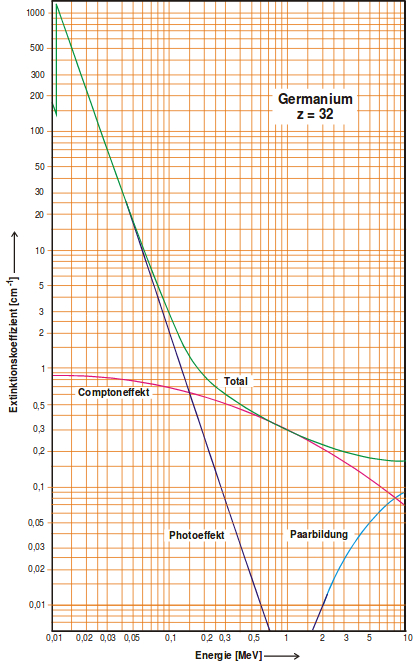
\includegraphics[width=0.3\textwidth]{Germanium.png}
    \caption{Energieabhängigkeit der einzellnen Wechselwirkungen von $\gamma$-Strahlung in
    einem Germaniumabsorber sowie die Totalabsorbtion \cite{anleitung}.}
    \label{abb:1}
\end{figure}
\subsection{Wechselwirkung von Beta-Strahlung mit Materie}
$\beta$-Stahlung besteht aus bei Kernprozessen freigewordenen Elektronen ($\beta^-$) bzw.
Positronen ($\beta^+$). Diese entstehen durch Umwandlung überschüssiger Neutronen bzw.
Protonen in instabilen Kernkonfigurationen. Die Umwandlungen finden dabei nach folgenden
Umwandlungsgleichungen statt:
\begin{align}
  \beta^- \, &: \, \symup{n} \rightarrow \symup{p} + \symup{e^-} + \symup{\bar{\nu}_e} \\
  \beta^+ \, &: \, \symup{p} \rightarrow \symup{n} + \symup{e^+} + \symup{\nu_e}.
\end{align}
Die Maximalenergie des $\beta$-Teilchens ist dabei die in diesem Prozess freiwerdende Energie,
diese muss aber nicht zwangsläufig komplett auf das $\beta$-Teilchen übertragen werden.
Das Energiespektrum ist daher im gegensatz zum $\gamma$-Quant kontinuierlich. Sowohl
das entstehende Kernteilchen sowie das (Anti-)Neutrino treten in keine Nennenswerte Wechselwirkung
mit dem bestrahlten Material. Im Gegensatz zum $\gamma$-Quant kann ein $\beta$-Teilchen
bei einem Durchgang durch die Absorberschicht weitaus mehr Wechselwirkungen erleiden,
was die Beschreibung durch ein Absorbtionsgesetz schwierig macht. Die Vielzahl der
Wechselwirkungen lässt sich dabei in die folgenden drei Prozesse einteilen:
\begin{enumerate}
  \item \textbf{Elastische Streuung an Atomkernen}: Die geladenen $\beta$-Teilchen
  treten dabei in das Coulomb-Feld der Atomkerne ein und werden daran abgelenkt.
  Dieser Prozess findet oft hintereinander statt, sodass das Teilchen einen weitaus längeren
  Weg durch die Materieschicht zurücklegt, als nur den theoretische Weg zwischen Quelle und
  Ende der Bahn (der sogenannten maximalen Reichweite $R_{\symup{max}}$).
  Die Richtungsänderung und damit die Streuung des Strahls ist dabei enorm,
  die Bremsung der einzellnen Teilchen aber nur gering.
  \item \textbf{Inelastische Streuung an Atomkernen}: In diesem Fall erfährt das Teilchen
  eine Beschleunigung durch das elektrostatische Feld des Atomkerns. Dabei muss
  Energie in Form von Strahlung abgegeben werden. Dieser Verlust in Form von \textbf{Bremsstrahlung}
  führt zu einer Abbremsung des Teilchens, für realistische Energien von $\beta$-Teilchen
  kann dadurch die beobachteten, bis zur kompletten Bremsung gehenden, Energieverluste
  jedoch nicht erklärt werden.
  \item \textbf{Inelastische Streuung an Elektronen}: Hiebei sorgen Stöße zwischen
  Elektronen des Absorbermaterials und den $\beta$-Teilchen für eine Anregung oder das vollständige
  Entfernen von Elektronen aus den Elektronenschalen der Absorberatome (Ionisation). Ein einzellner
  solcher Stoß führt nur zu geringen Energieverlusten, ein $\beta$-Teilchen führt jedoch
  viele solcher Stöße hintereinander aus, sodass bereits geringe Plattendicken zu vollständiger
  Abbremsung der Teilchen bewirkt, insbesondere bei Platten aus schweren Elementen
  mit dementsprechend vielen Elektronen.
\end{enumerate}
Da es nicht vorherzusagen ist, welche dieser Stoßprozesse das $\beta$-Teilchen tatsächlich
durchführt, kann kein allgemeingültiges Absorbtionsgesetz angegeben werden. Werden jedoch
nicht zu dicke Schichten Absorbermaterial sowie Strahler, bei denen die Energieverteilung
statistisch (siehe Abbildung \ref{abb:2}) ist genommen, ist ein Absorbtionsgesetz wie \ref{eqn:1} in guter Näherung gültig.
Die Absorbtionskurve verhält sich dann wie in Abbildung \ref{abb:3} dargestellt. Durch
schneiden der linearen Verlängerung des anfänglichen Abfalls der Intensität mit der
Untergrundstrahlung kann ein guter Näherungswert für $R_\symup{max}$ gewonnen werden,
aus dem sich nach folgender empirisch gewonnenen Formel die Maximalenergie der
emmitierten Teilchen bestimmen lässt:
\begin{equation}
  E_\symup{max} = 1.92 \sqrt{R_\symup{max}^2 + 0.22 R_\symup{max}} \; [\si{\mega\electronvolt}],
  \label{eqn:3}
\end{equation}
wobei $R_\symup{max}$ einer Massenbelegung (Einheit: \si{\gram\per\square\centi\metre})
entspricht.
\begin{figure}
  \centering
  \begin{subfigure}{0.4\textwidth}
    \centering
      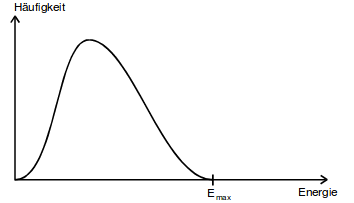
\includegraphics[width=\textwidth]{betaspektrum.png}
      \caption{Kontinuierliches Emmisionsspektrum eines $\beta$-Strahler \cite{anleitung}.}
      \label{abb:2}
  \end{subfigure}
  \begin{subfigure}{0.4\textwidth}
    \centering
      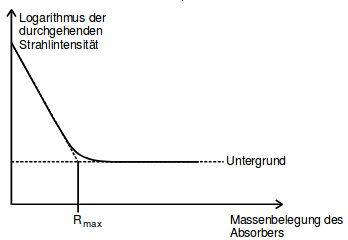
\includegraphics[width=\textwidth]{betafit.png}
      \caption{Absorbtionskure für einen $\beta$-Strahler, die lineare Weiterführung
      ist gestrichelt angedeutet \cite{anleitung}.}
      \label{abb:3}
  \end{subfigure}
  \caption{}
\end{figure}
\section{Durchführung}
\subsection{Versuchsaufbau}
Der Versuchsaufbau besteht aus einem in einer Abschirmung angebrachten Geiger-Müller-Zählrohr,
das in gerader Linie auf die Strahlenquelle gerichtet ist. Zwischen Strahlenquelle und Zählrohr
können in einem Plattenwagen Absorberplatten unterschiedlicher Dicke angebracht werden.
Die Messzeit des Zählrohrs lässt sich dabei in Sekunden einstellen und variieren.
Als Strahlenquelle für die Messung mit $\gamma$-Strahlung wird eine $\ce{^{137}Cs}$-Probe verwendet,
für die mit $\beta$-Strahlung eine $\ce{^{99}Tc}$-Probe.
\begin{figure}
  \centering
    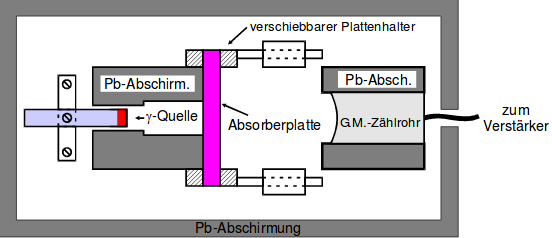
\includegraphics[width=0.6\textwidth]{aufbau.png}
    \caption{Skizze des Versuchsaufbaus \cite{anleitung}.}
    \label{abb:4}
\end{figure}
\subsection{Versuchsdurchführung}
Zuerst werden die Dicken der Platten mit einer Schiebelehre vermessen sowie die Nullraten
an den Zählrohren für \SI{1000}{\second} gemessen. Dann werden für verschiedene Plattendicken
und Materialien ($\ce{Cu}$, $\ce{Zn}$ bei $\gamma$-Strahlung sowie $\ce{Pb}$ und $\ce{Fe}$
bei $\beta$-Strahlung)
die Zählraten an den Geiger-Müller-Zählrohren gemessen, die Zähldauer wird wenn nötig
erhöht um auswertbare Daten zu erhalten. Die Platten werden dabei kombiniert und eng
aneinander gedrückt, um höhere Dicken zu erreichen.
\section{Auswertung}
\subsection{Bestimmung der Absoprtionskoeffizienten}
Für den Absorptionskoeffizient von Kupfer gilt \SI[per-mode=reciprocal]{2.77(15)e5}{\per\metre}
\begin{table}
  \centering
  \begin{tabular}{c c c}
    \toprule
     & Zink & Kupfer \\
    \midrule
    N(0) / \si[per-mode=reciprocal]{\per\second} & \num{139.8(29)} & \num{144.6(11)}  \\
    $\mu$ / \si[per-mode=reciprocal]{\per\metre} & \num{47.3(17)} & \num{63.0(12)} \\
    \bottomrule
  \end{tabular}
  \caption{Ergebnisse.}
  \label{tab:1}
\end{table}

\begin{figure}
  \begin{subfigure}{0.5\textwidth}
    \centering
    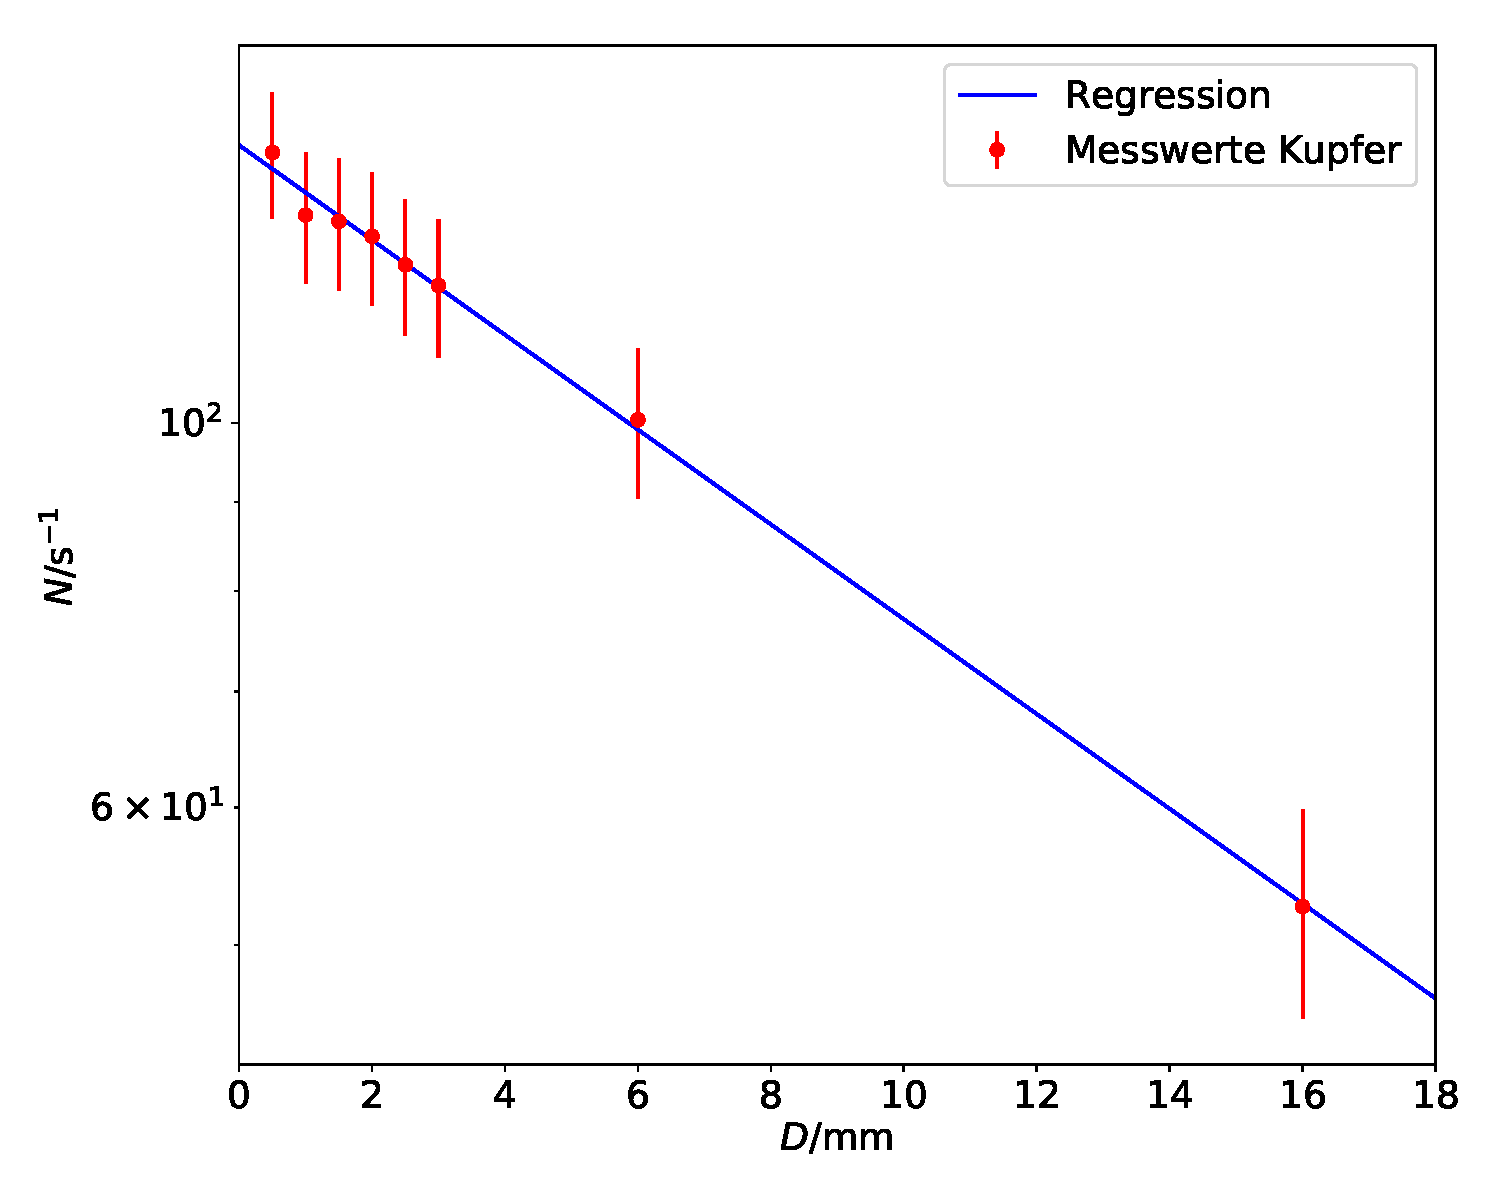
\includegraphics[width=\textwidth]{CuGamma.pdf}
    \caption{Messwerte von Kupfer mit Regression.}
    \label{sub:1}
  \end{subfigure}
  \begin{subfigure}{0.5\textwidth}
    \centering
    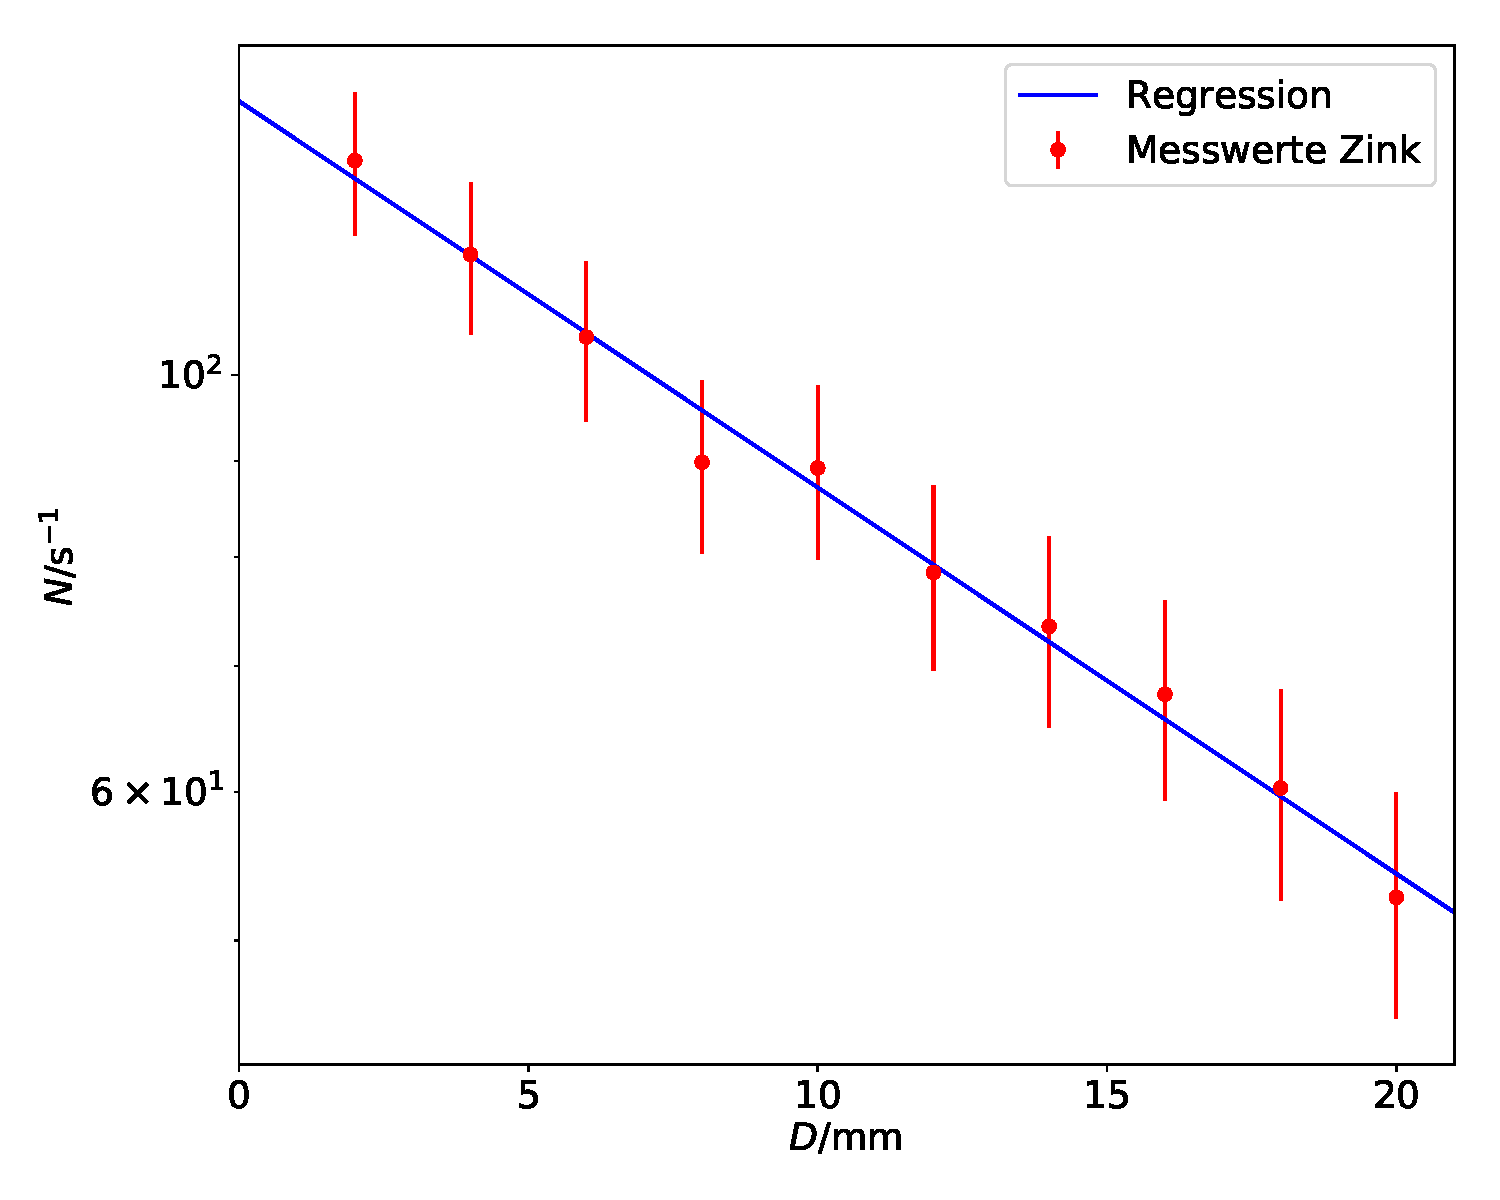
\includegraphics[width=\textwidth]{ZnGamma.pdf}
    \caption{Messwerte von Zink.}
    \label{sub:2}
  \end{subfigure}
  \caption{Ergebnisse.}
  \label{fig:1}
\end{figure}

\section{Diskussion}
\newpage
\nocite{*}
\printbibliography
